%! TEX program = xelatex

%===========================================================================%
%->> Project: hitszthesis_master
%->> Author: Lazyshawn
%->> Coding: UTF-8
%->> Contact: 20s053030@stu.hit.edu.cn
%->> More: https://github.com/lazyshawn/hitszthesis.git
%===========================================================================%

% ==>> 模板设置
% []: midterm 中期模板 | 空 毕业论文模板
% {}: style/thesis_master 硕士模板 | style/thesis_doctor 博士模板
\documentclass[midterm]{style/thesis_doctor}
% \documentclass{style/thesis_doctor}

% ==>> 导言区设置
%! TEX root = ./main.tex

% ===== 论文信息填写 =====
% 中文标题
\zhtitle{基于视觉与触觉反馈的在手操作研究}{标题第二行}
% 英文标题
\entitle{IN-HAND MANIPULATION BASED ON VISUAL AND TACTICLE FEEDBACK}
% 作者姓名: 中文+英文
\author{胡韶}{Hu Shao}
% 学号
\studentid{20S053030}
% 导师姓名: 中文+英文
\teacher{刘云辉}{Liu Yunhui}
% 学院
\department{机电工程与自动化学院}
% 专业
\speciality{机械工程}
% 答辩日期: 中文+英文
\defensedate{2020年3月}{June, 2020}
% 入学时间
\enrollment{2016年9月}


% \includeonly{main/abstract, main/introduction}

\usepackage{lipsum}  % 随机文本,测试用

% ==>> 毕业论文模板
% \begin{document}
%   % ===== Cover | 封面 =====
%   \maketitle
%
%   % ===== Front | 书前部分 =====
%   \frontmatter
%   % --- Abstract / 摘要 ---
%   %! TEX root = ../main.tex

\begin{abstract}
在本项目中,实验目的是使用平行指夹具控制工具在重力作用下按照规定的轨迹达到目标位置。
本文从运动过程中系统的物理学模型、对应的控制方法、实验方案、
仿真实验设计和具体实验操作等方面展开,
研究并验证单自由度机械手利用重力实现在手操作的实现方法。

我们从理论角度分析了工具运动过程中的物理现象,
假设摩擦模型仅包含库伦摩擦力和粘滞摩擦力,在此基础上建立起动力学模型。
我们参照非线性控制中的模型参考自适应控制系统建立了控制模型,
并阐述了其基本原理和作用,推导了系统的控制方程和调参律。
从实验的角度再次分析该问题,
我们设计了可实践的伺服控制算法和基于改良 PD 控制策略的力控算法,
并通过实验验证其合理性。
最后使用 MATLAB/Simulik 的多体动力学模块进行了仿真实验,
实验结果表明使用模型参考自适应控制后,在部分物理参数如工具质量、
摩擦系数等未知的情况下,该控制系统仍然能正常运行,
工具能在重力作用下依照指定的轨迹运动到期望位置。

本文的研究结果意味着,通过使用合适的控制策略,
结构简单、抓取方式单一的平行指夹具也可以实现复杂的在手操作动作,
其在实际生产线上可以有更广阔的应用范围。

\keyword{在手操作;非线性控制;模型参考自适应控制;改良PD控制算法;伺服控制;多体动力学仿真}
\end{abstract}

\begin{enabstract}
In this project, the robot with a parallel gripper holds the tool with a pinch grasp.
In this work, we study and verfy how a rather simple gripper can still perfom in-hand-manipulations via making full using of gravity.
We show these in various ways, such as the mechanical modeling,
design of controll algorithm, scheduling experiment, simulation, and so on.

The grasp only affords friction against gravity,
such that tool can slides as planning by suitable control the grasp force.
From a theoretical point, we analyse the physical phenomenon in processing this action.
We then formulate the sliding dynamics,
by modeling the friction as Coulomb and viscous friction.
We model the control system and formulate the standard adaptive control law,
refering to the nonlinear control system.
Experimentally, we design a practical servo-control algorithm and
modified PD control algorithm, which are verified in experiment.
At last, we simulate in Simscape multibody,
which is one simulation block of MATLAB/Simulink.
The experimental results show, the proposed adaptation law can
compensate for parametric error to some extent, and manage to slide the tool.

The results of this study mean that even a rather simple gripper can still perfom in- hand-manipulations,
when the control scheme is designed appropriately.
By this way, gripper with single degree of freedom can have wider applications in the future.

\enkeyword{In-hand manipulation, Nonlinear control, Adaptive control,  \par
Improved PD control algorithm, Servo control, Simscape Multibody}
\end{enabstract}


%   % --- Contents / 目录 ----
%   \tableofcontents
%   \tableofencontents  % (博士)英文目录
%
%   % ===== Main | 正文部分 =====
%   \mainmatter
%
%   % --- Main body | 正文 ---
%   %! TEX root = ../main.tex

\chapter{绪论}
\section{课题背景及研究的目的和意义}
这是\LaTeX 中的一段中文\cite{man}。

\lipsum[1]

\nocite{*}


%   %! TEX root = ../main.tex

\chapter{常用环境的使用}
\section{公式}
牛顿第二定律描述了物体的动量和所受外力之间的关系,
动量为$p$的质点,在外力$F$的作用下,
其动量随时间的变化率同该质点所受的外力成正比,并与外力的方向相同。
牛顿第二定律的数学表述如式(\ref{equ:Newton_2})所示。
\begin{equation}
  F_e=\frac{d}{dt}mv;
  \label{equ:Newton_2}
\end{equation}

\begin{note}
  \para{$F_e$}{物体所受合外力(N);\hfill{}}
  \para{$m$}{物体质量(kg);}
  \para{$v$}{物体运动速度($\rm{m/s^2}$)。}
\end{note}

通常,物体质量不随时间变化,因此牛顿第二定律也可表述为$F_e=ma$。


\section{插图}
图\ref{fig:HK}是一个包含四个子图的浮动体。
图\ref{subfig1-1}$\sim$ \ref{subfig1-3}是三个插入题注的子图,
而第四个子图不插入题注。

\begin{figure}[!ht]
\centering
  \subfloat[子图1\label{subfig1-1}]{
    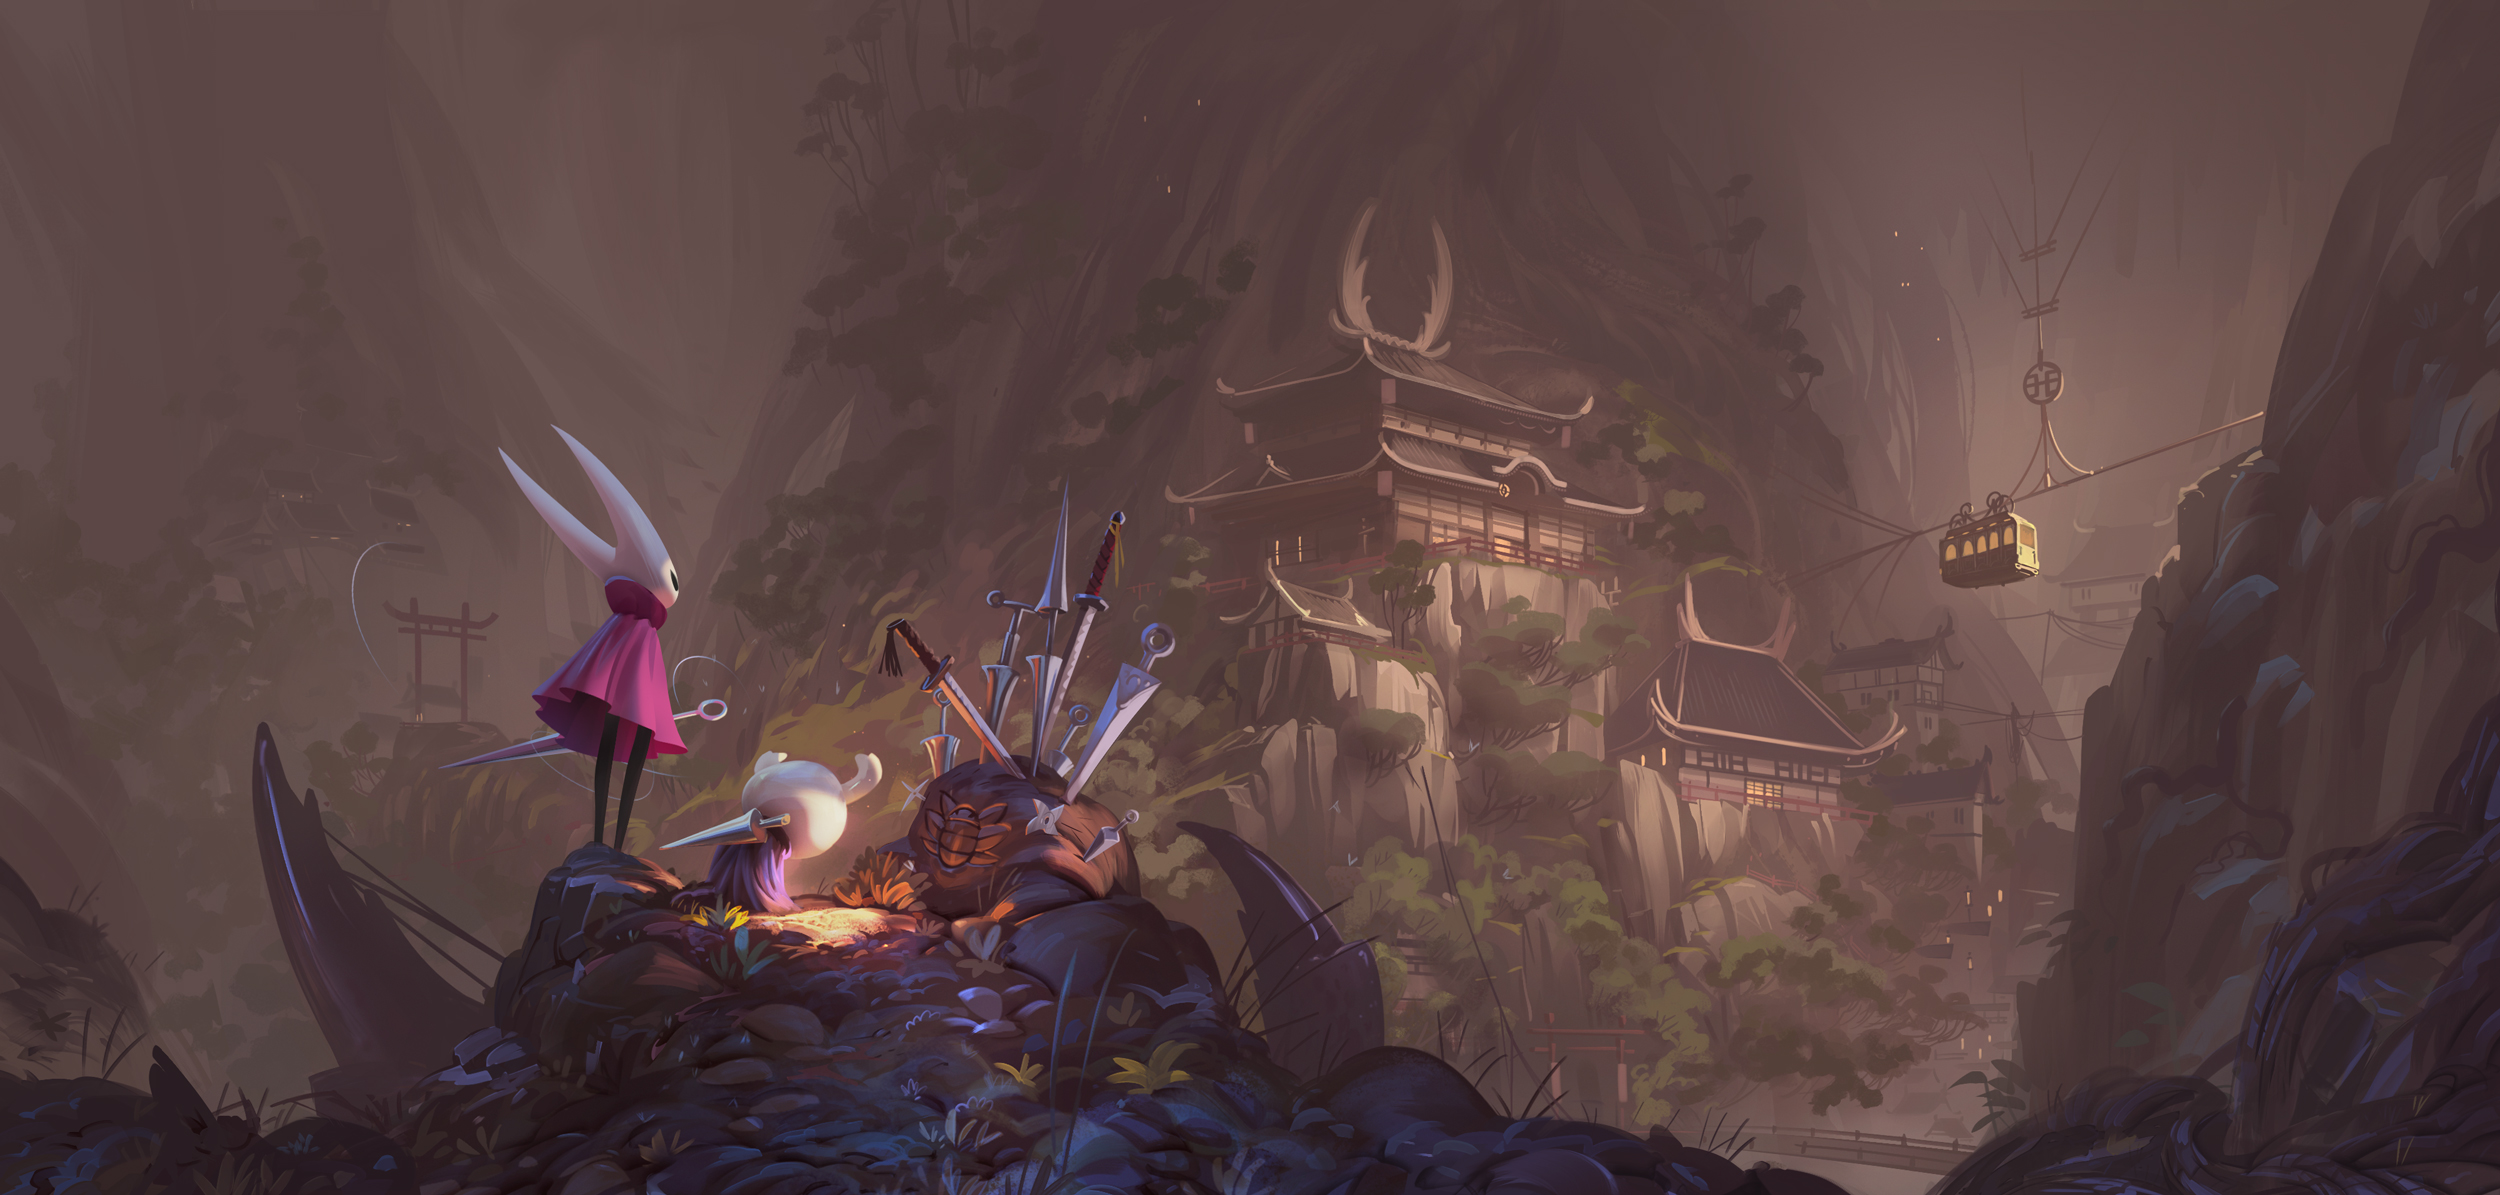
\includegraphics[scale=0.07]{pics/pic.jpg}
    % \setcounter{subfigure}{0}  % 子图序号计数器
  }
  \hspace{30pt}
  \subfloat[子图2\label{subfig1-2}]{
    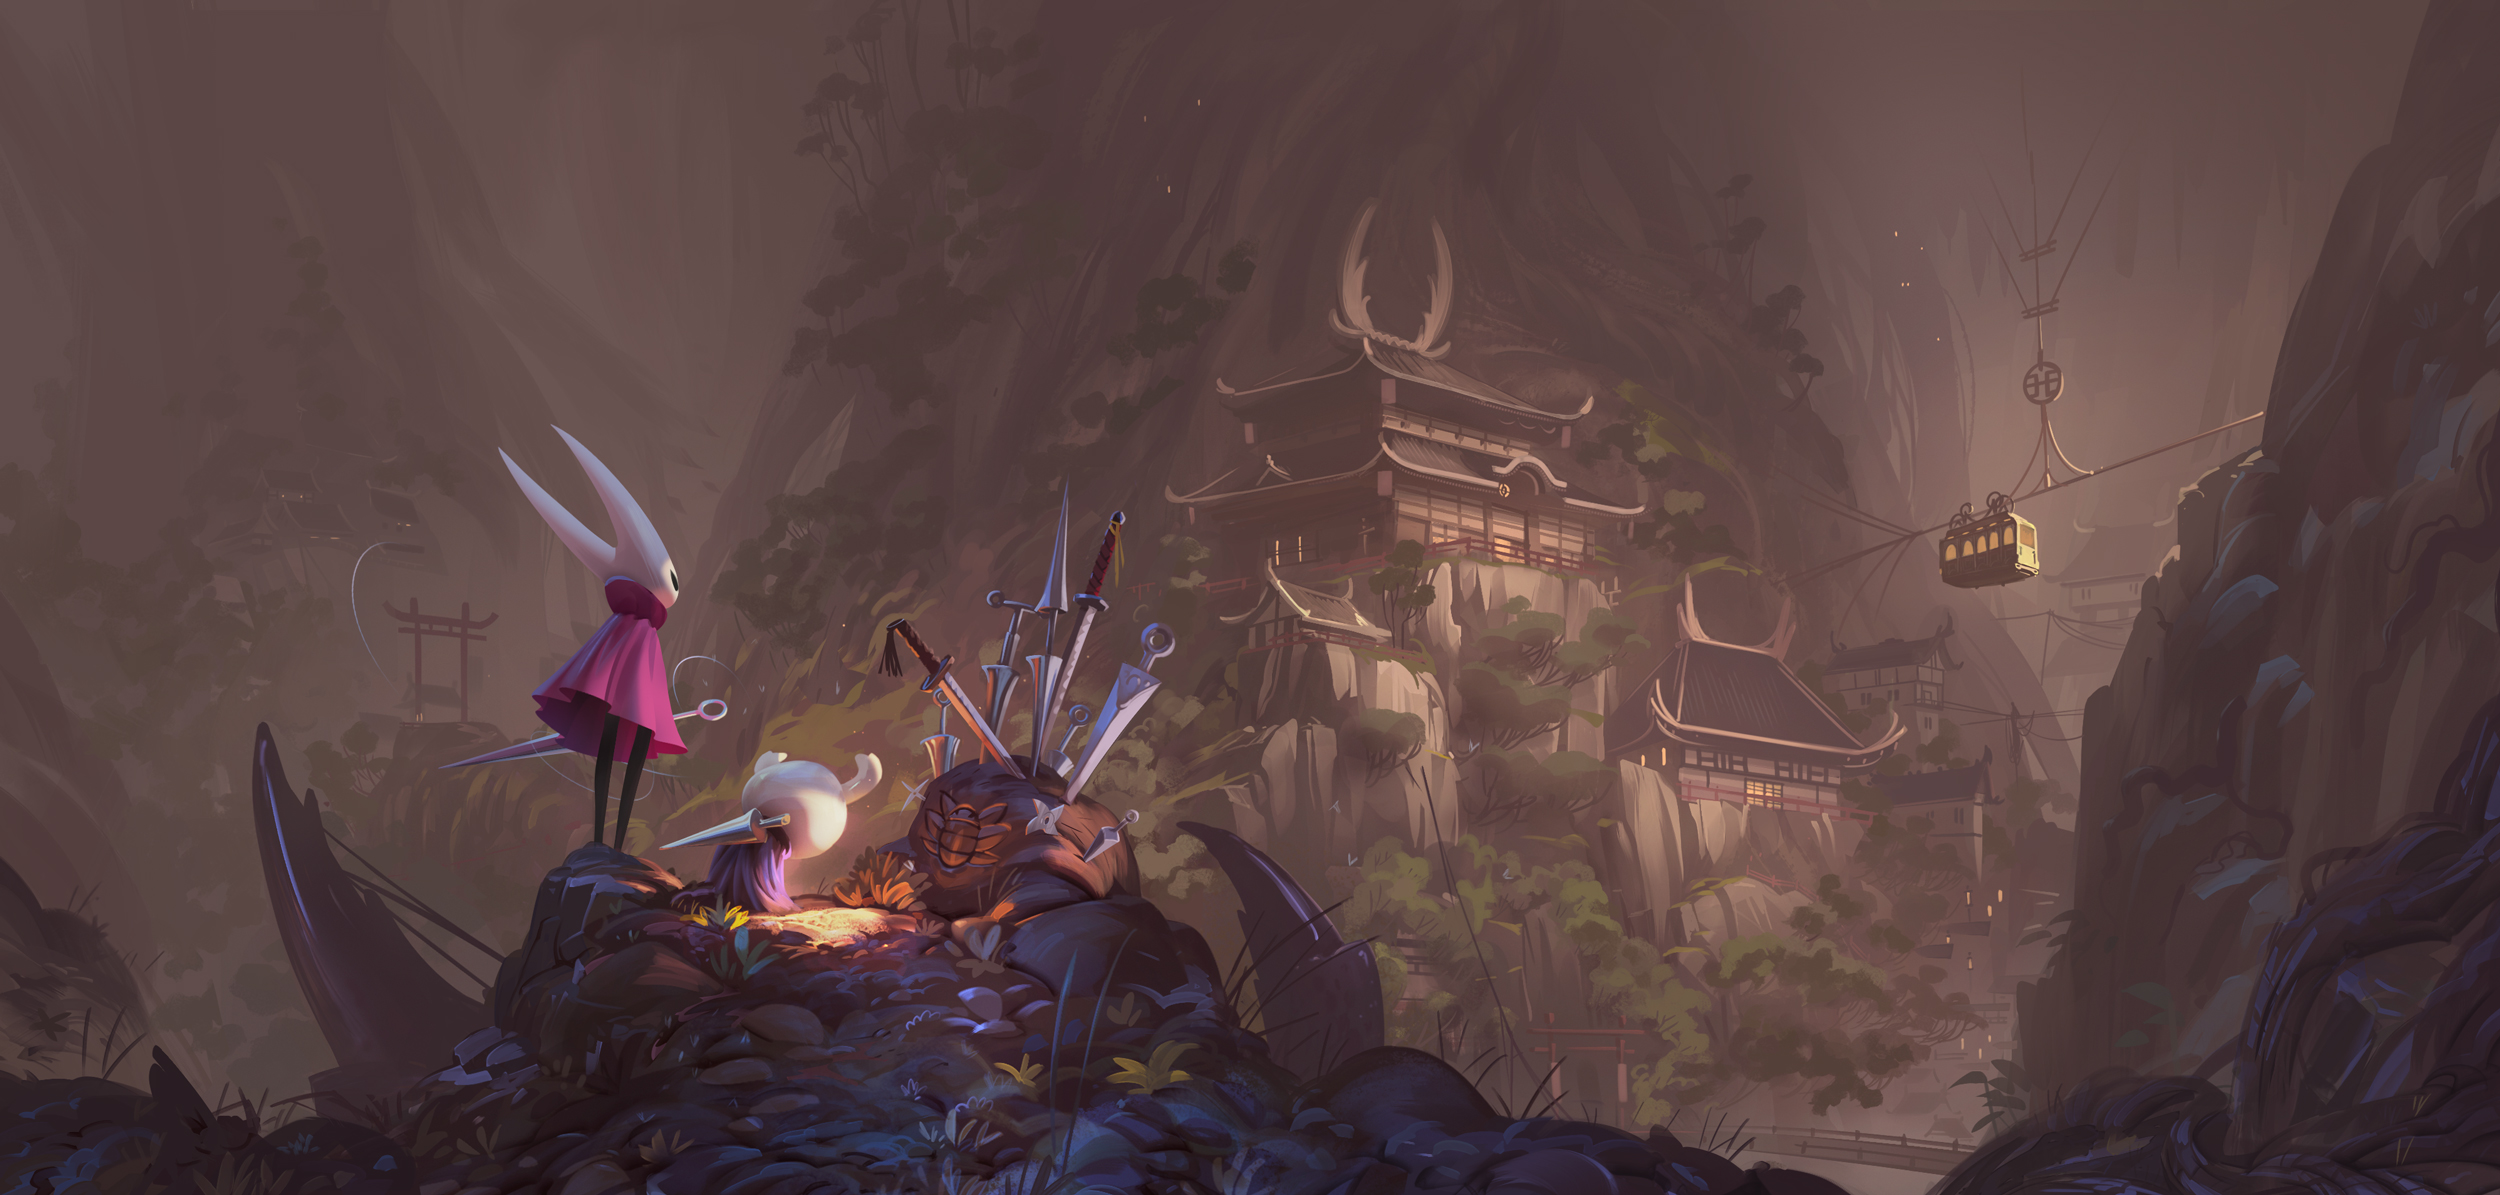
\includegraphics[scale=0.07]{pics/pic.jpg}
  } \\
  \subfloat[子图3\label{subfig1-3}]{
    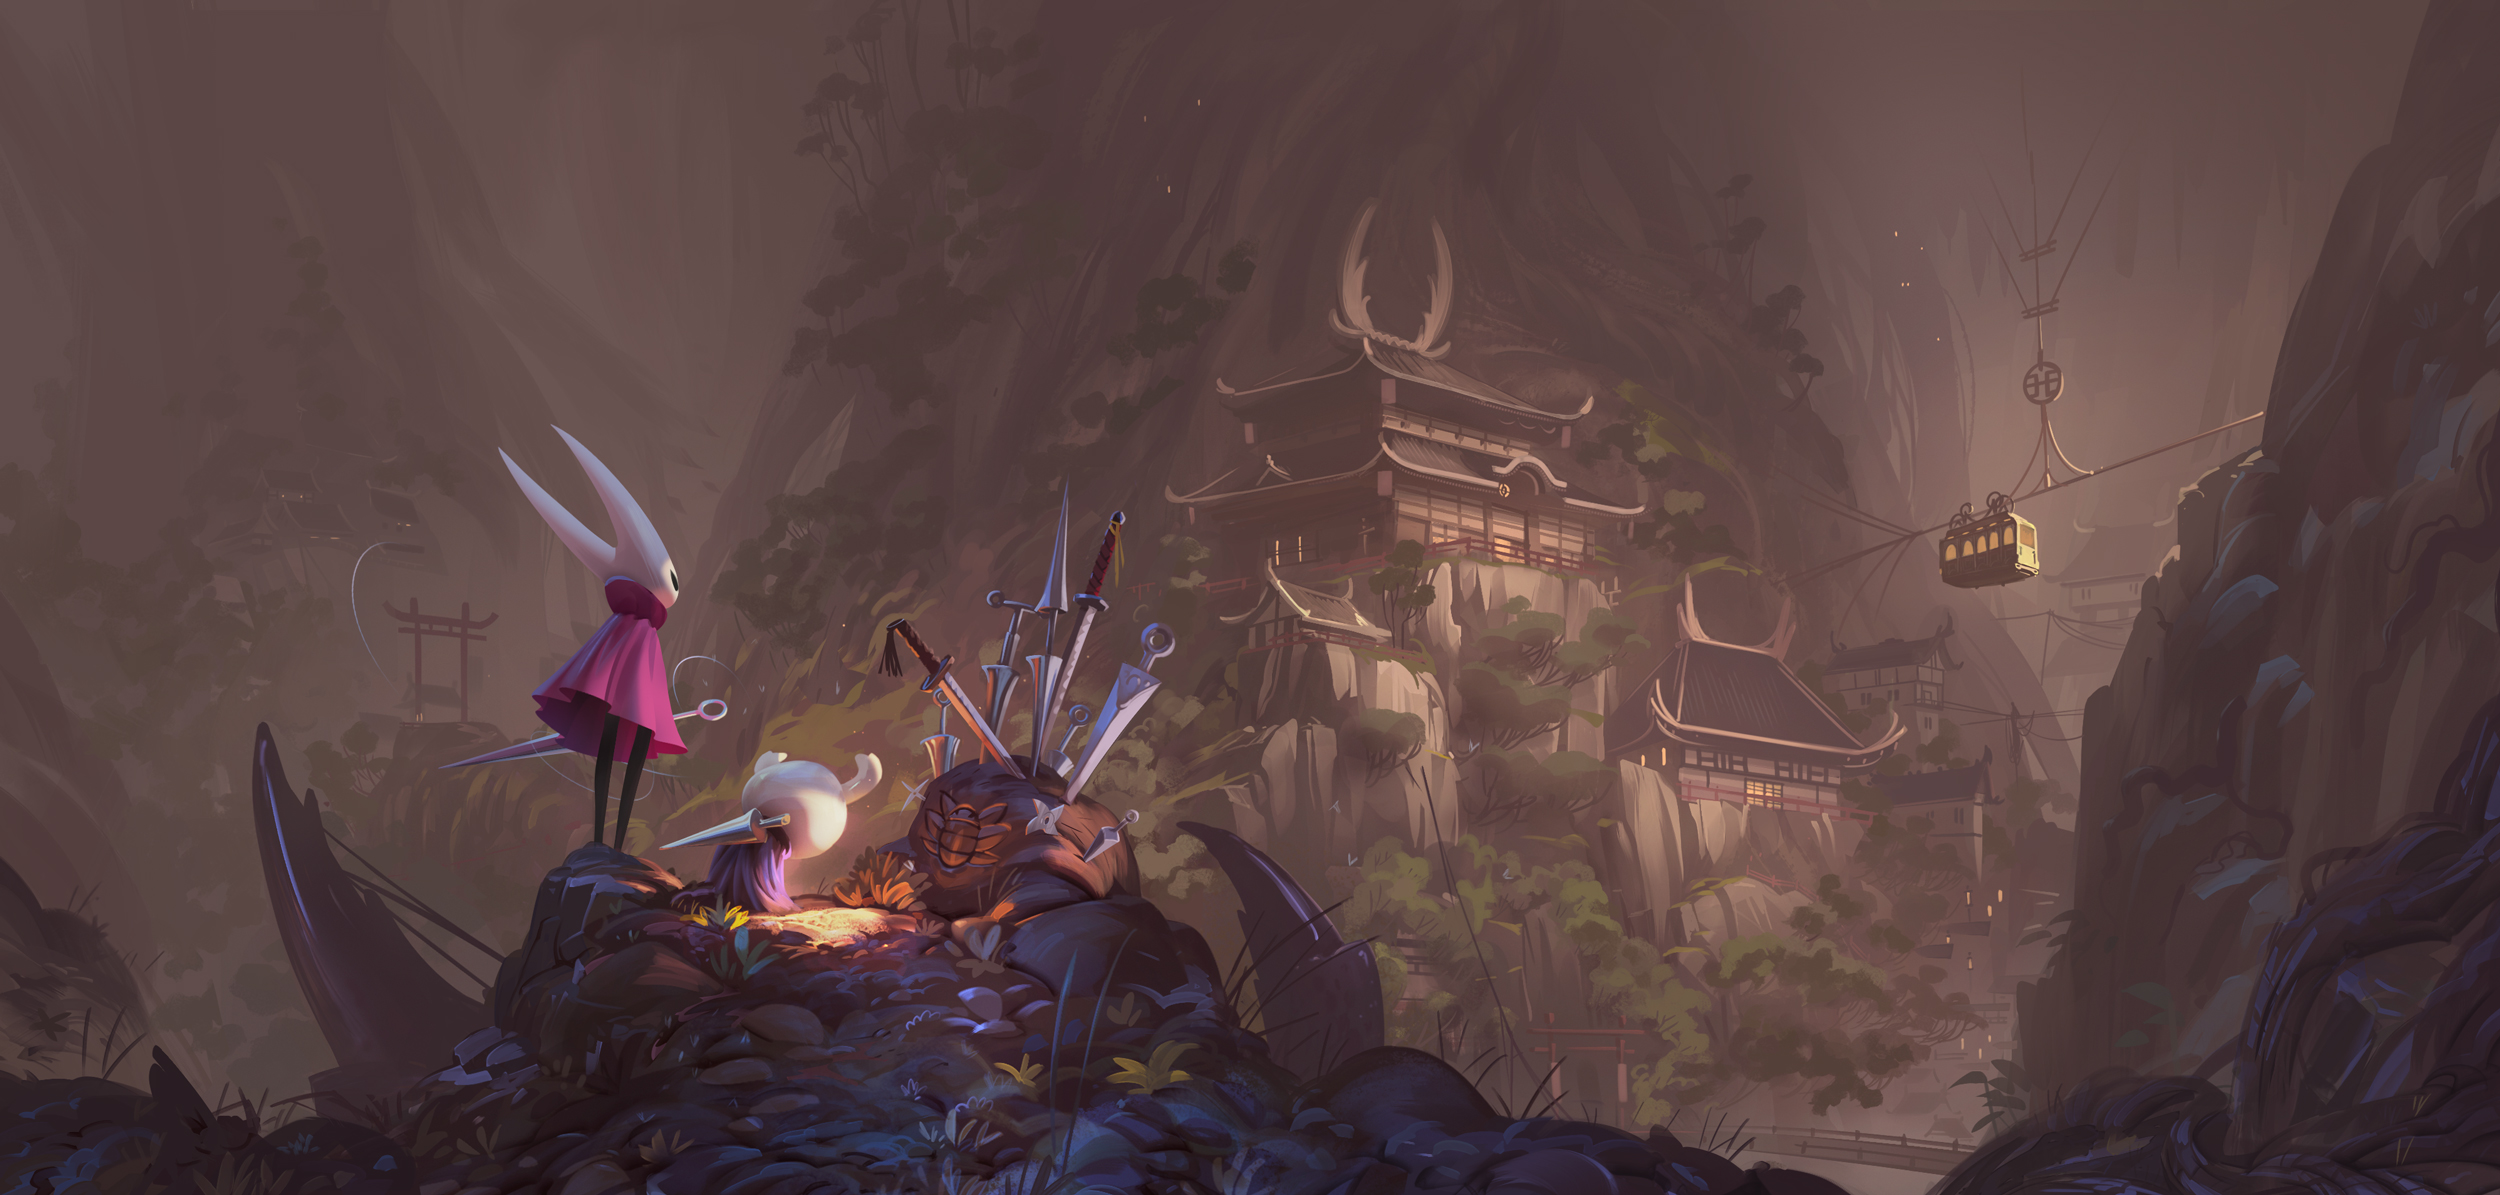
\includegraphics[scale=0.07]{pics/pic.jpg}
  }
  \hspace{30pt}
  \subfloat{
    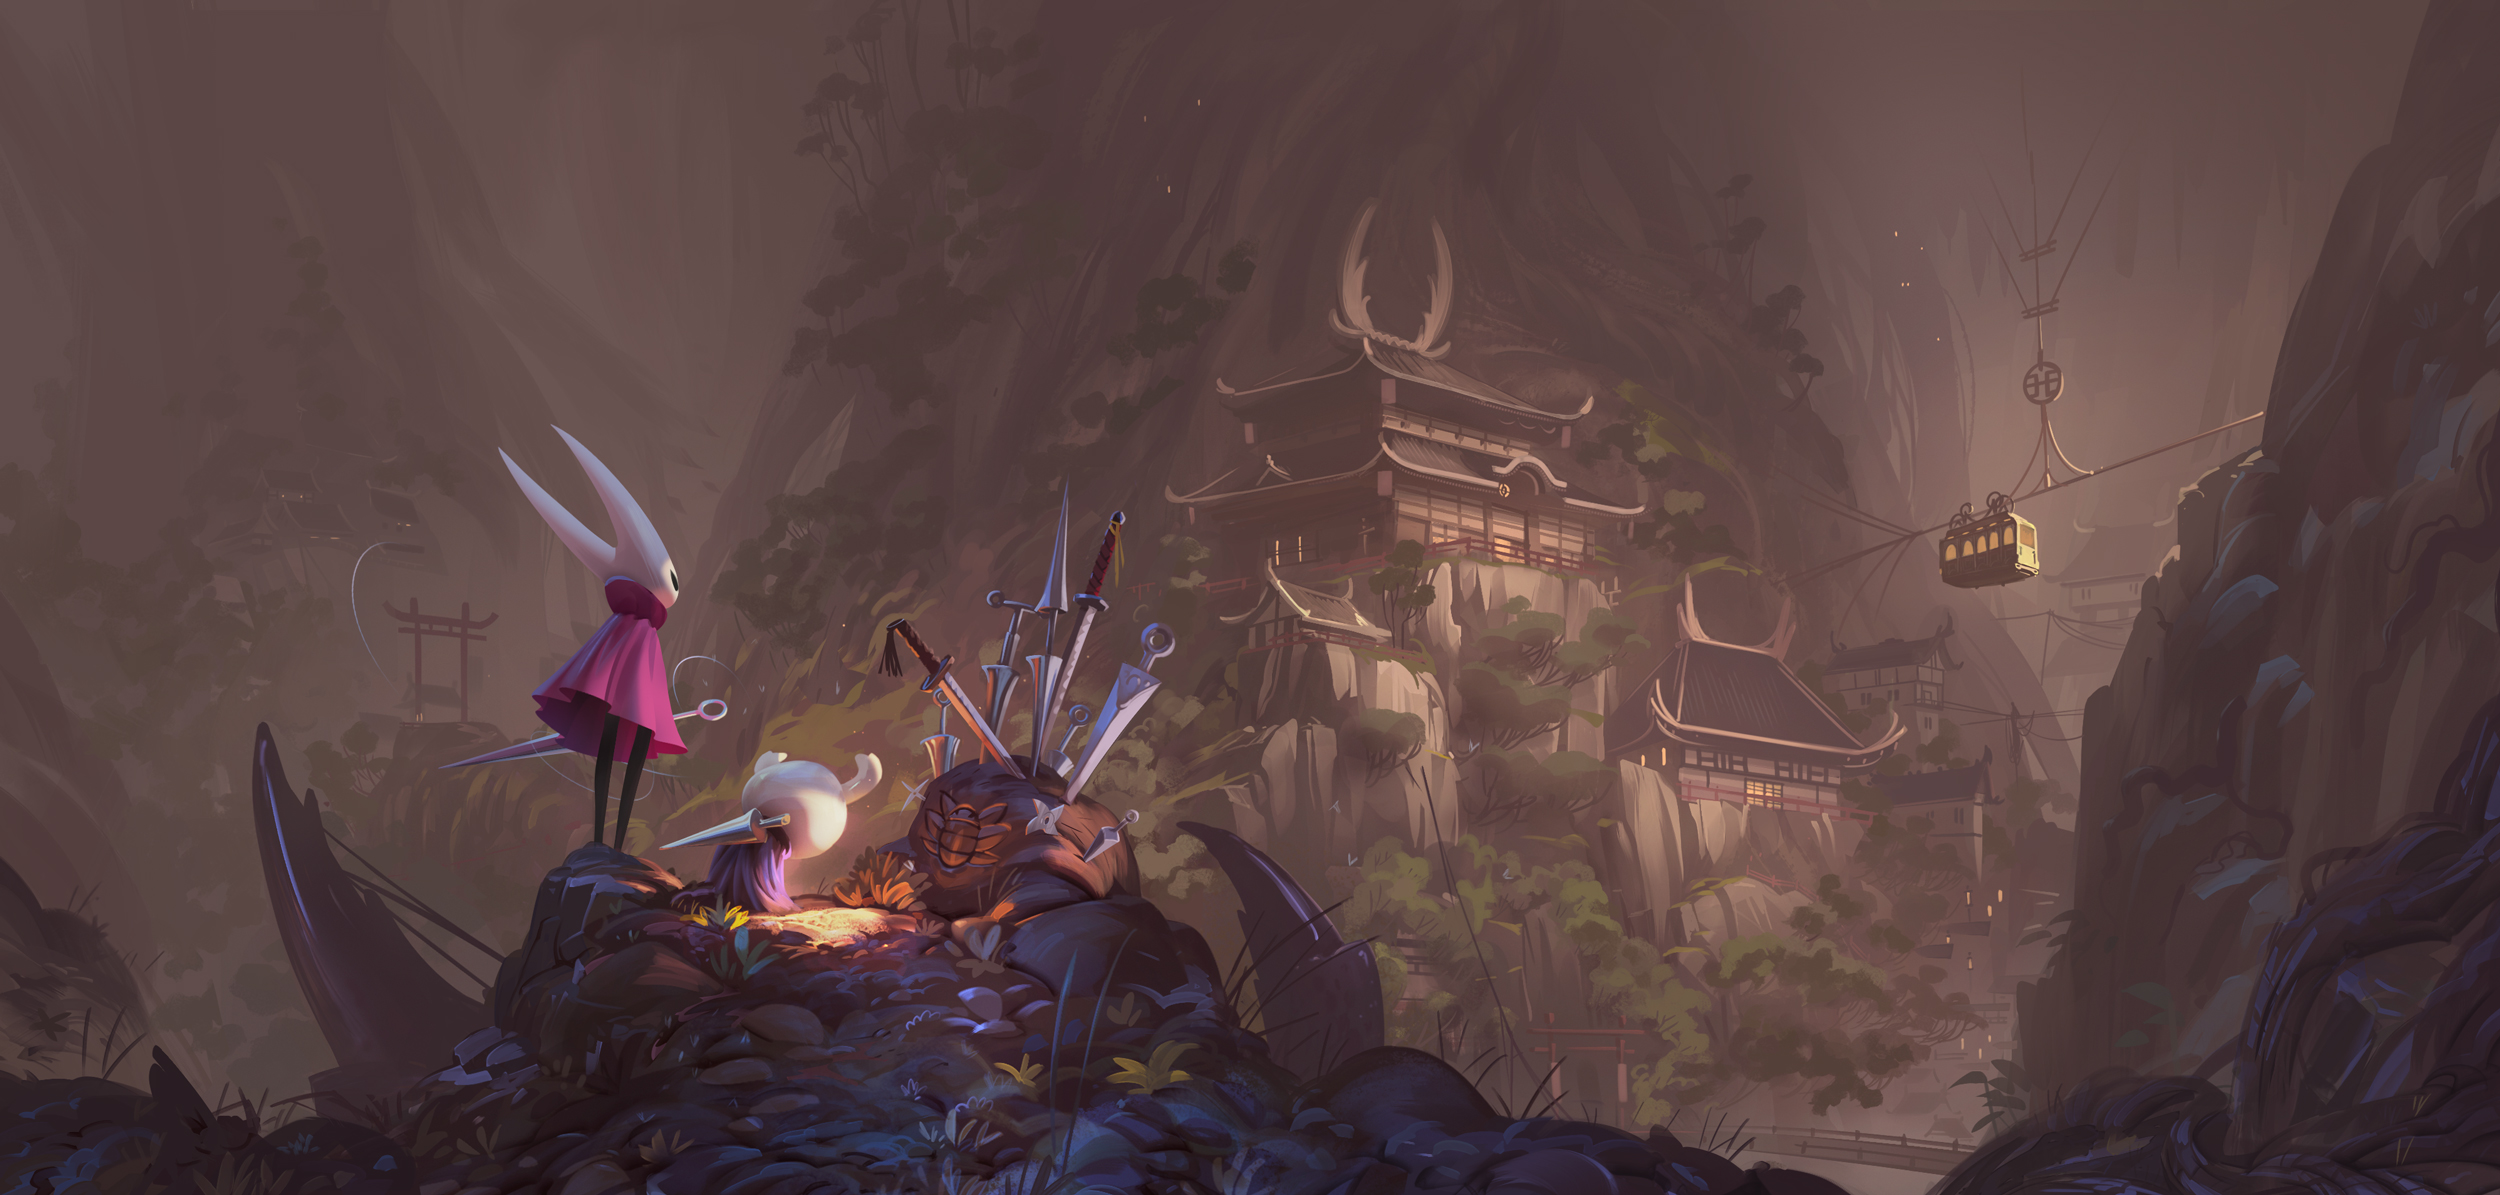
\includegraphics[scale=0.07]{pics/pic.jpg}
}
\caption{Hollow Knight}
\label{fig:HK}
\vspace{-0.3cm}
\end{figure}


\section{表格}
三线表的绘制。很多刊物都明确规定稿件中要使用三线表。三线表在必要时也可添加若干条水平辅助分隔中线。
\begin{table}[!h]
\centering
\caption{序号计数器及其用途\label{tab:2-1}}
\begin{tabular}{@{}ll@{}}
\toprule[1pt]
计数器名   & 用途            \\ \midrule
chapter    & 章序号计数器    \\
section    & 节序号计数器    \\
subsection & 小节序号计数器  \\
\bottomrule[1pt]
\end{tabular}
\end{table}

表\ref{tab:2-1}中列出了常用章节的计数器名称。

\section{列表}
排序列表
\begin{enumerate}
  \item item of the list.
  \item item of the list.
  \item item of the list.
\end{enumerate}



%   %! TEX root = ../main.tex

\begin{conclusion}
本课题的研究内容主要是从运动过程中系统的物理学模型、对应的控制方法、
实验方案、仿真实验设计和具体实验操作等方面展开,
研究并验证单自由度机械手利用重力实现在手操作的实现方法。
本文主要研究的工作总结如下:

\begin{enumerate}
  \item 分析了单自由度机器人手在手操作过程中物体的运动规律。
    对摩擦模型进行了假设, 用滑动摩擦力和粘滞摩擦力来近似表示物体
    在滑动临界点和正常运动时的摩擦力。根据牛顿定律得到物体运动过程中的动力学模型,
    分析夹爪施加给物体的正压力和物体运动状态之间的关系。
  \item 建立夹爪和被控物体系统的控制方程。根据物体运动过程中的动力学方程
    分析了在手操作的控制难点在于摩擦力的估计和考虑被控物体质量的可变性。
    参照模型参考自适应控制理论推到了系统的自适应控制方程,
    以夹爪施加的正压力为系统输入控制工具的运动状态,
    使得系统在摩擦系数未知的情况下可以对不同质量的工具进行在手操作。
  \item 分析系统控制方程, 设计控制方案。
    本研究设计并改良PD控制算法来控制夹爪施加给物体的正压力,
    保证系统控制输入量与控制方程一致。
    采用伺服控制来实现高频率运动, 保证控制操作精度。
    通过C++多线程编程协调伺服控制、力控、数据采集与处理等进程的时间安排。
  \item 设计仿真和实验方案, 验证自适应控制算法的准确性。
    调试和校准了实验设备, 并进行夹爪的在手操作实验, 实验结果不符合预期,
    原因是自适应控制参数设置不合理, 且出现了积分饱和现象。
    为此本项目使用Simulink仿真软件验证控制方程的正确性, 在此基础上搭建系统的仿真模型,
    验证了控制方案的合理性。
    同时仿真结果表明使用自适应控制后,在摩擦系数和物体质量未知的情况下,
    该控制系统仍然能正常运行,依照指定的轨迹运动到期望位置。
\end{enumerate}

针对单自由度机器人手利用重力对工具进行手上操作的实现方法这一问题,
本文先从理论角度分析了工具运动过程中的物理现象,对摩擦模型进行了假设,
建立起动力学模型。
为了建立合适的控制模型,我们选择使用模型参考自适应控制系统来建立控制模型,
并阐述了其基本原理和作用,推导了系统的控制方程和调参律。
从实验的角度分析该问题,我们设计了可实践的伺服控制算法和力控算法,
并通过实验验证该算法的合理性。
最后进行了仿真实验,实验结果验证了单自由度机器人手用于在手操作的可行性;
同时表明使用模型参考自适应控制后,在部分物理参数未知的情况下,
该控制系统仍然能正常运行,依照指定的轨迹运动到期望位置。

本文的研究结果意味着,通过使用合适的控制策略,
结构简单、抓取方式单一的平行指夹具也可以实现复杂的在手操作动作,
在实际生产线上可以有更广阔的应用范围。

鉴于时间和个人能力有限,本项目目前的实验结果尚不理想,这可能影响到本文的严谨性。
后续的工作将会继续展开,之后的主要内容是完成一系列严谨的实验,
进一步验证平行指夹具进行手上操作方面的可能性,并实现更复杂的操作。

\end{conclusion}

%   % --- Reference | 参考文献 ---
%   \nocite{*} % 测试用
%   \bibliography{refs/reference}
%   % --- Publication | 发表的论文 ---
%   \publication

\section*{(一)发表的学术论文}
\begin{listSquare}
  \item {\Large$\times \times \times$, $\times \times \times$}. 
    Static Oxidation Model of Al-Mg/C Dissipation Thermal Protection 
    Materials[J]. Rare Metal Materials and Engineering,
    2010, 39(Suppl. 1): 520-524. (SCI收录, IDS号为669JS, IF=0.16)
  \item {\Large$\times \times \times$, $\times \times \times$}. 
    局部多孔质气体静压轴向轴承静态特性的数值求解[J].
    摩擦学学报, 2007 (1): 68-72. (EI收录号: 20071510544816)
\end{listSquare}

% 无专利时此项不必列出
\section*{(二)申请及已获得的专利}

\section*{(三)参与的科研项目及获奖情况}



%   % --- Authorization | 原创性声明 ---
%   \authorization
%   % --- Acknowledgment | 致谢 ---
%   %! TEX root = ../main.tex

\begin{acknowledgement}
本论文设计在姜欣老师的悉心指导和严格要求下业已完成,
从课题选取到具体的写作过程,从论文初稿到定稿姜老师都一直悉心指导,
在我的毕业设计期间,姜老师为我带给了种种专业知识上的指导和一些富于创造性的推荐。
没有这样的指导和帮助,我不会这么顺利的完成毕业设计。
在此向姜欣老师表示深深的感谢和崇高的敬意!

我也要感谢赵杰师兄在科研工作之余抽出时间为我解答疑难。
在我的科研实验和写作过程中,赵杰师兄对我提出了许多宝贵的意见,
也帮我开拓研究思路。师兄的无私帮助和热忱鼓励,让我毕业设计完成更顺利,
真诚地向赵杰师兄表示感谢。

同时我也要感谢我的同学们,他们的关爱和无私帮忙使得我度过艰难,成功地
完成所有任务。
\end{acknowledgement}

%   % --- Resume | 个人简历 ---
%   \resume


%
%
%   % ===== Appendix | 附录 =====
%   % \appendix
%   % %! TEX root = ../main.tex

\chapter{Appendx 1}
\appchapter{附录第一章}
\appsection{课题背景}
\lipsum[3]


%   % \includepdf[pages={1,2}]{appendices/article.pdf}
% \end{document}

% ==>> 中期模板
\begin{document}
  % ===== Cover | 封面 =====
  \maketitle

  % ===== Front | 书前部分 =====
  \frontmatter

  % ===== Main | 正文部分 =====
  \mainmatter

  % --- Main body | 正文 ---
  %! TEX root = ../main.tex

\chapter{绪论}
\section{课题背景及研究的目的和意义}
这是\LaTeX 中的一段中文\cite{man}。

\lipsum[1]

\nocite{*}


  %! TEX root = ../main.tex

\chapter{常用环境的使用}
\section{公式}
牛顿第二定律描述了物体的动量和所受外力之间的关系,
动量为$p$的质点,在外力$F$的作用下,
其动量随时间的变化率同该质点所受的外力成正比,并与外力的方向相同。
牛顿第二定律的数学表述如式(\ref{equ:Newton_2})所示。
\begin{equation}
  F_e=\frac{d}{dt}mv;
  \label{equ:Newton_2}
\end{equation}

\begin{note}
  \para{$F_e$}{物体所受合外力(N);\hfill{}}
  \para{$m$}{物体质量(kg);}
  \para{$v$}{物体运动速度($\rm{m/s^2}$)。}
\end{note}

通常,物体质量不随时间变化,因此牛顿第二定律也可表述为$F_e=ma$。


\section{插图}
图\ref{fig:HK}是一个包含四个子图的浮动体。
图\ref{subfig1-1}$\sim$ \ref{subfig1-3}是三个插入题注的子图,
而第四个子图不插入题注。

\begin{figure}[!ht]
\centering
  \subfloat[子图1\label{subfig1-1}]{
    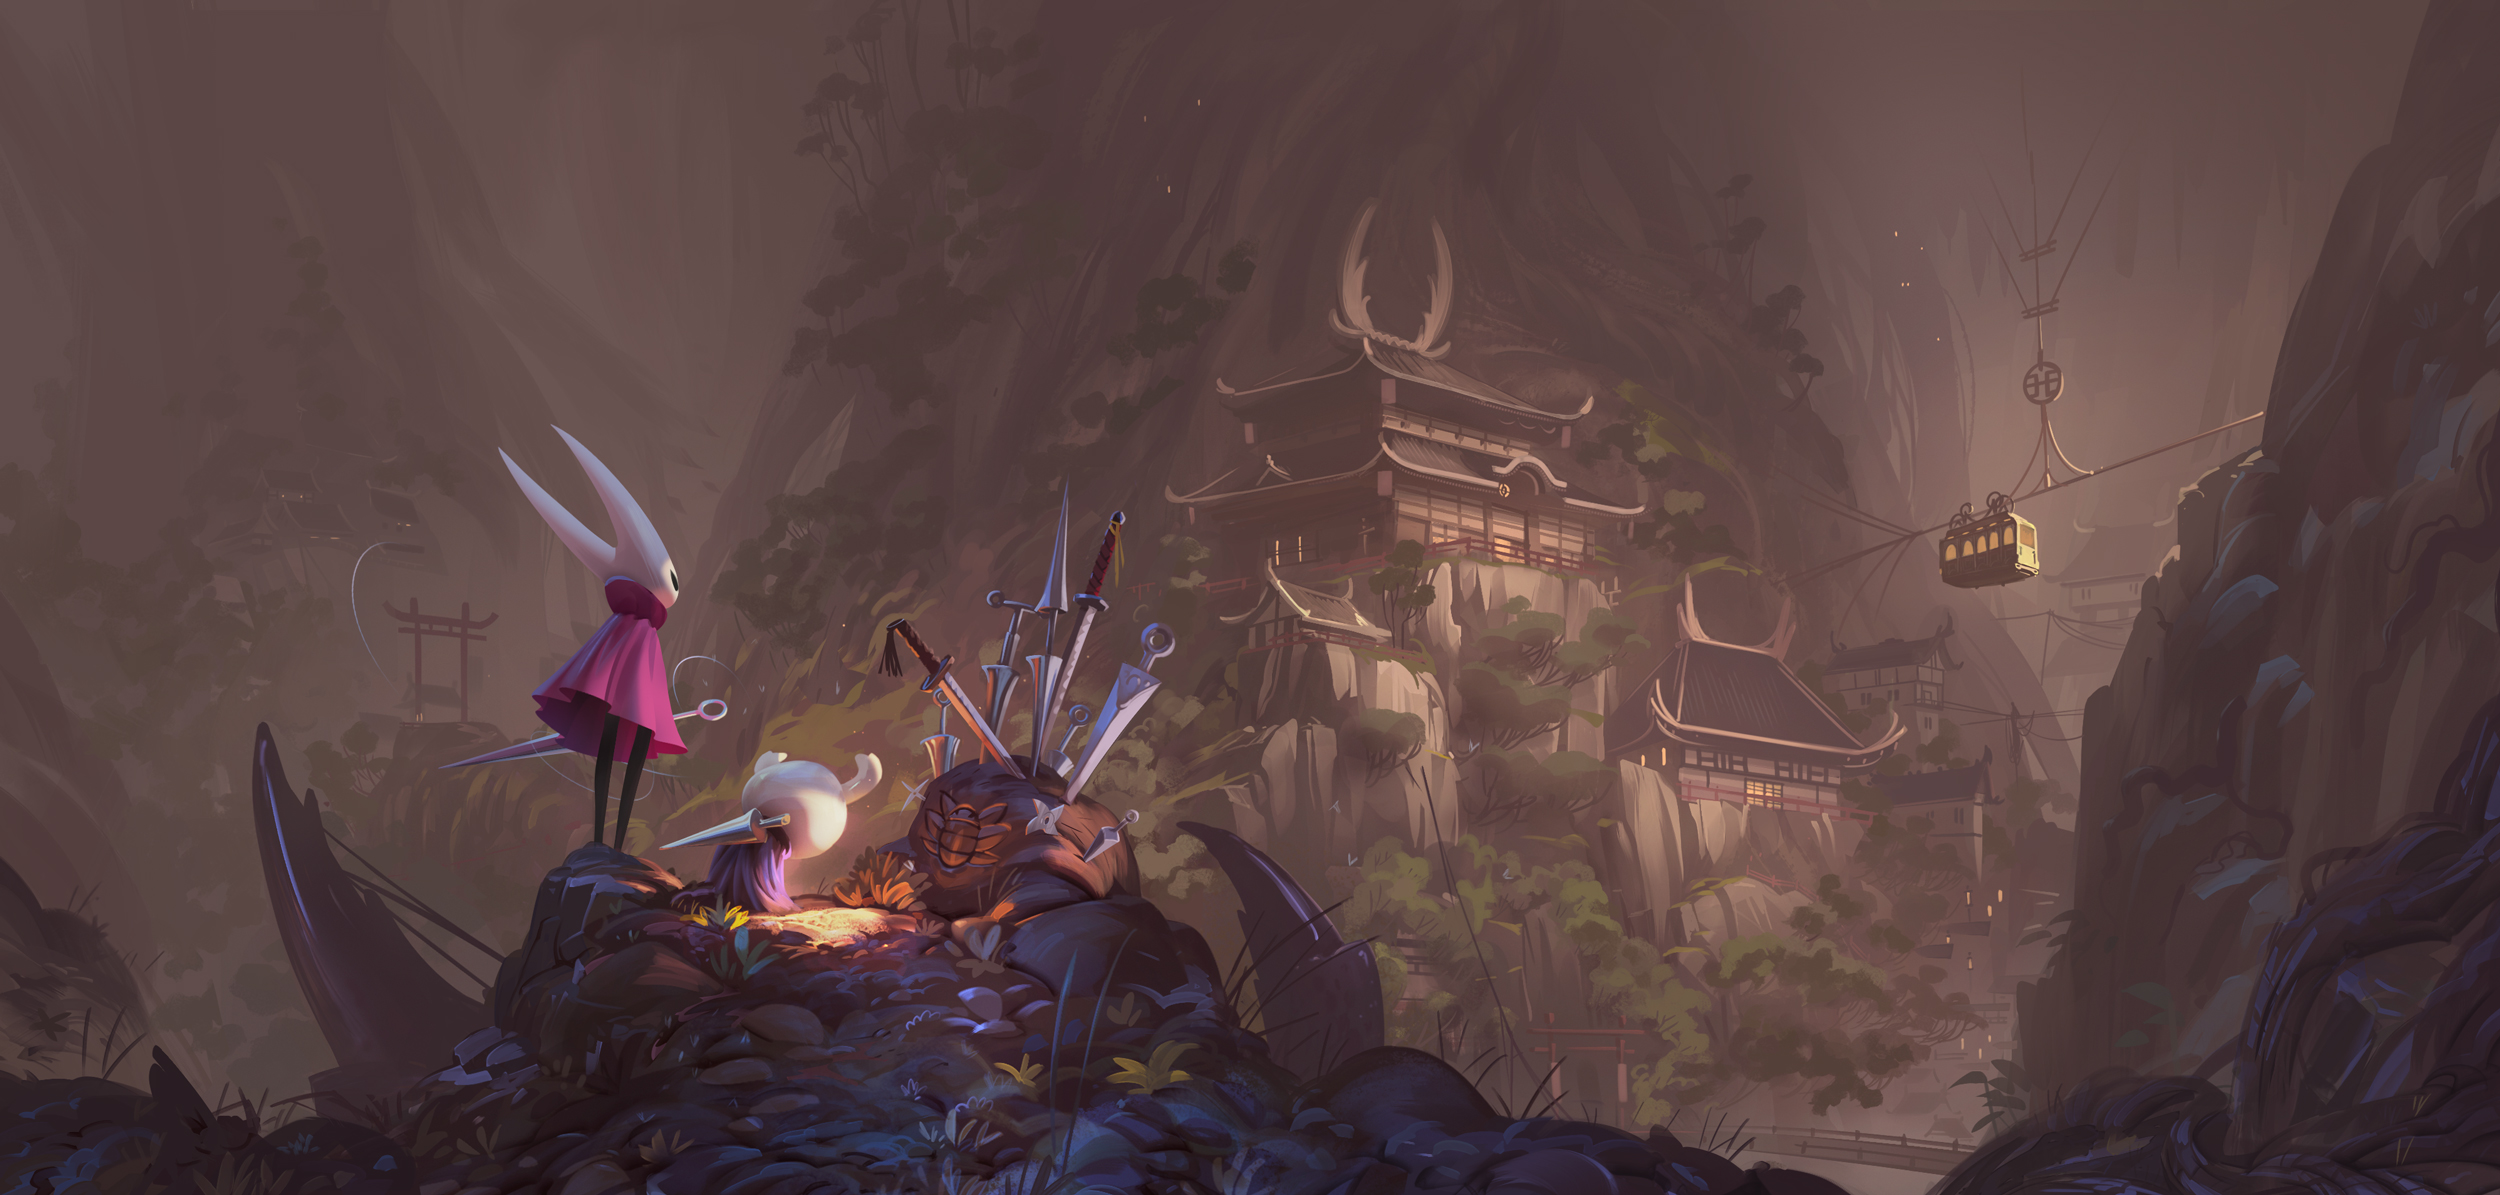
\includegraphics[scale=0.07]{pics/pic.jpg}
    % \setcounter{subfigure}{0}  % 子图序号计数器
  }
  \hspace{30pt}
  \subfloat[子图2\label{subfig1-2}]{
    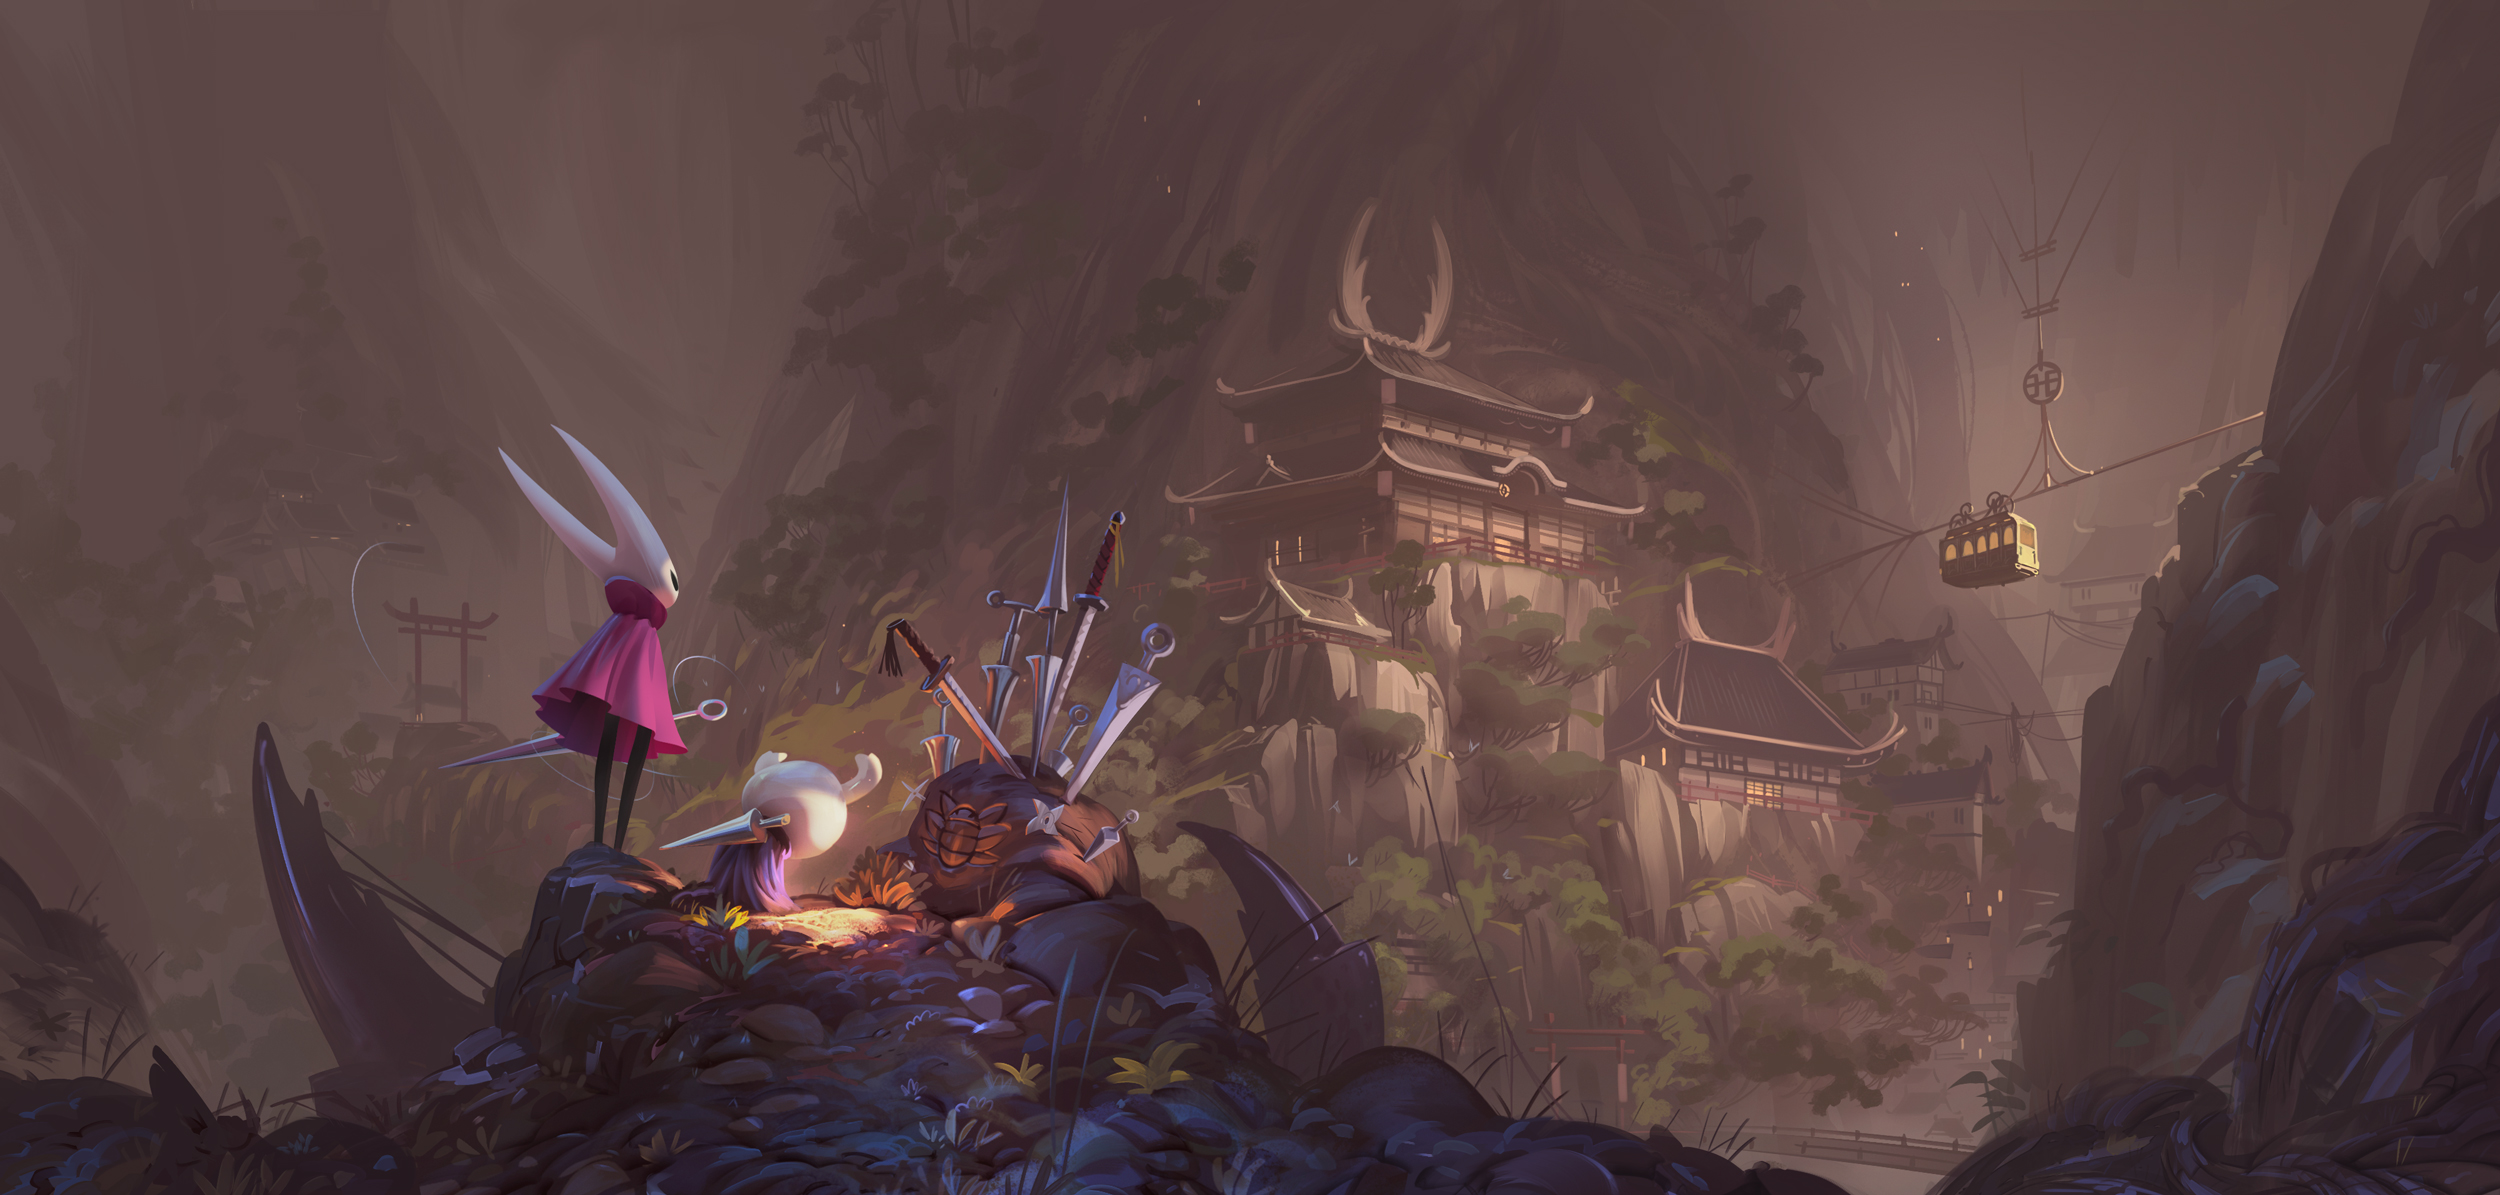
\includegraphics[scale=0.07]{pics/pic.jpg}
  } \\
  \subfloat[子图3\label{subfig1-3}]{
    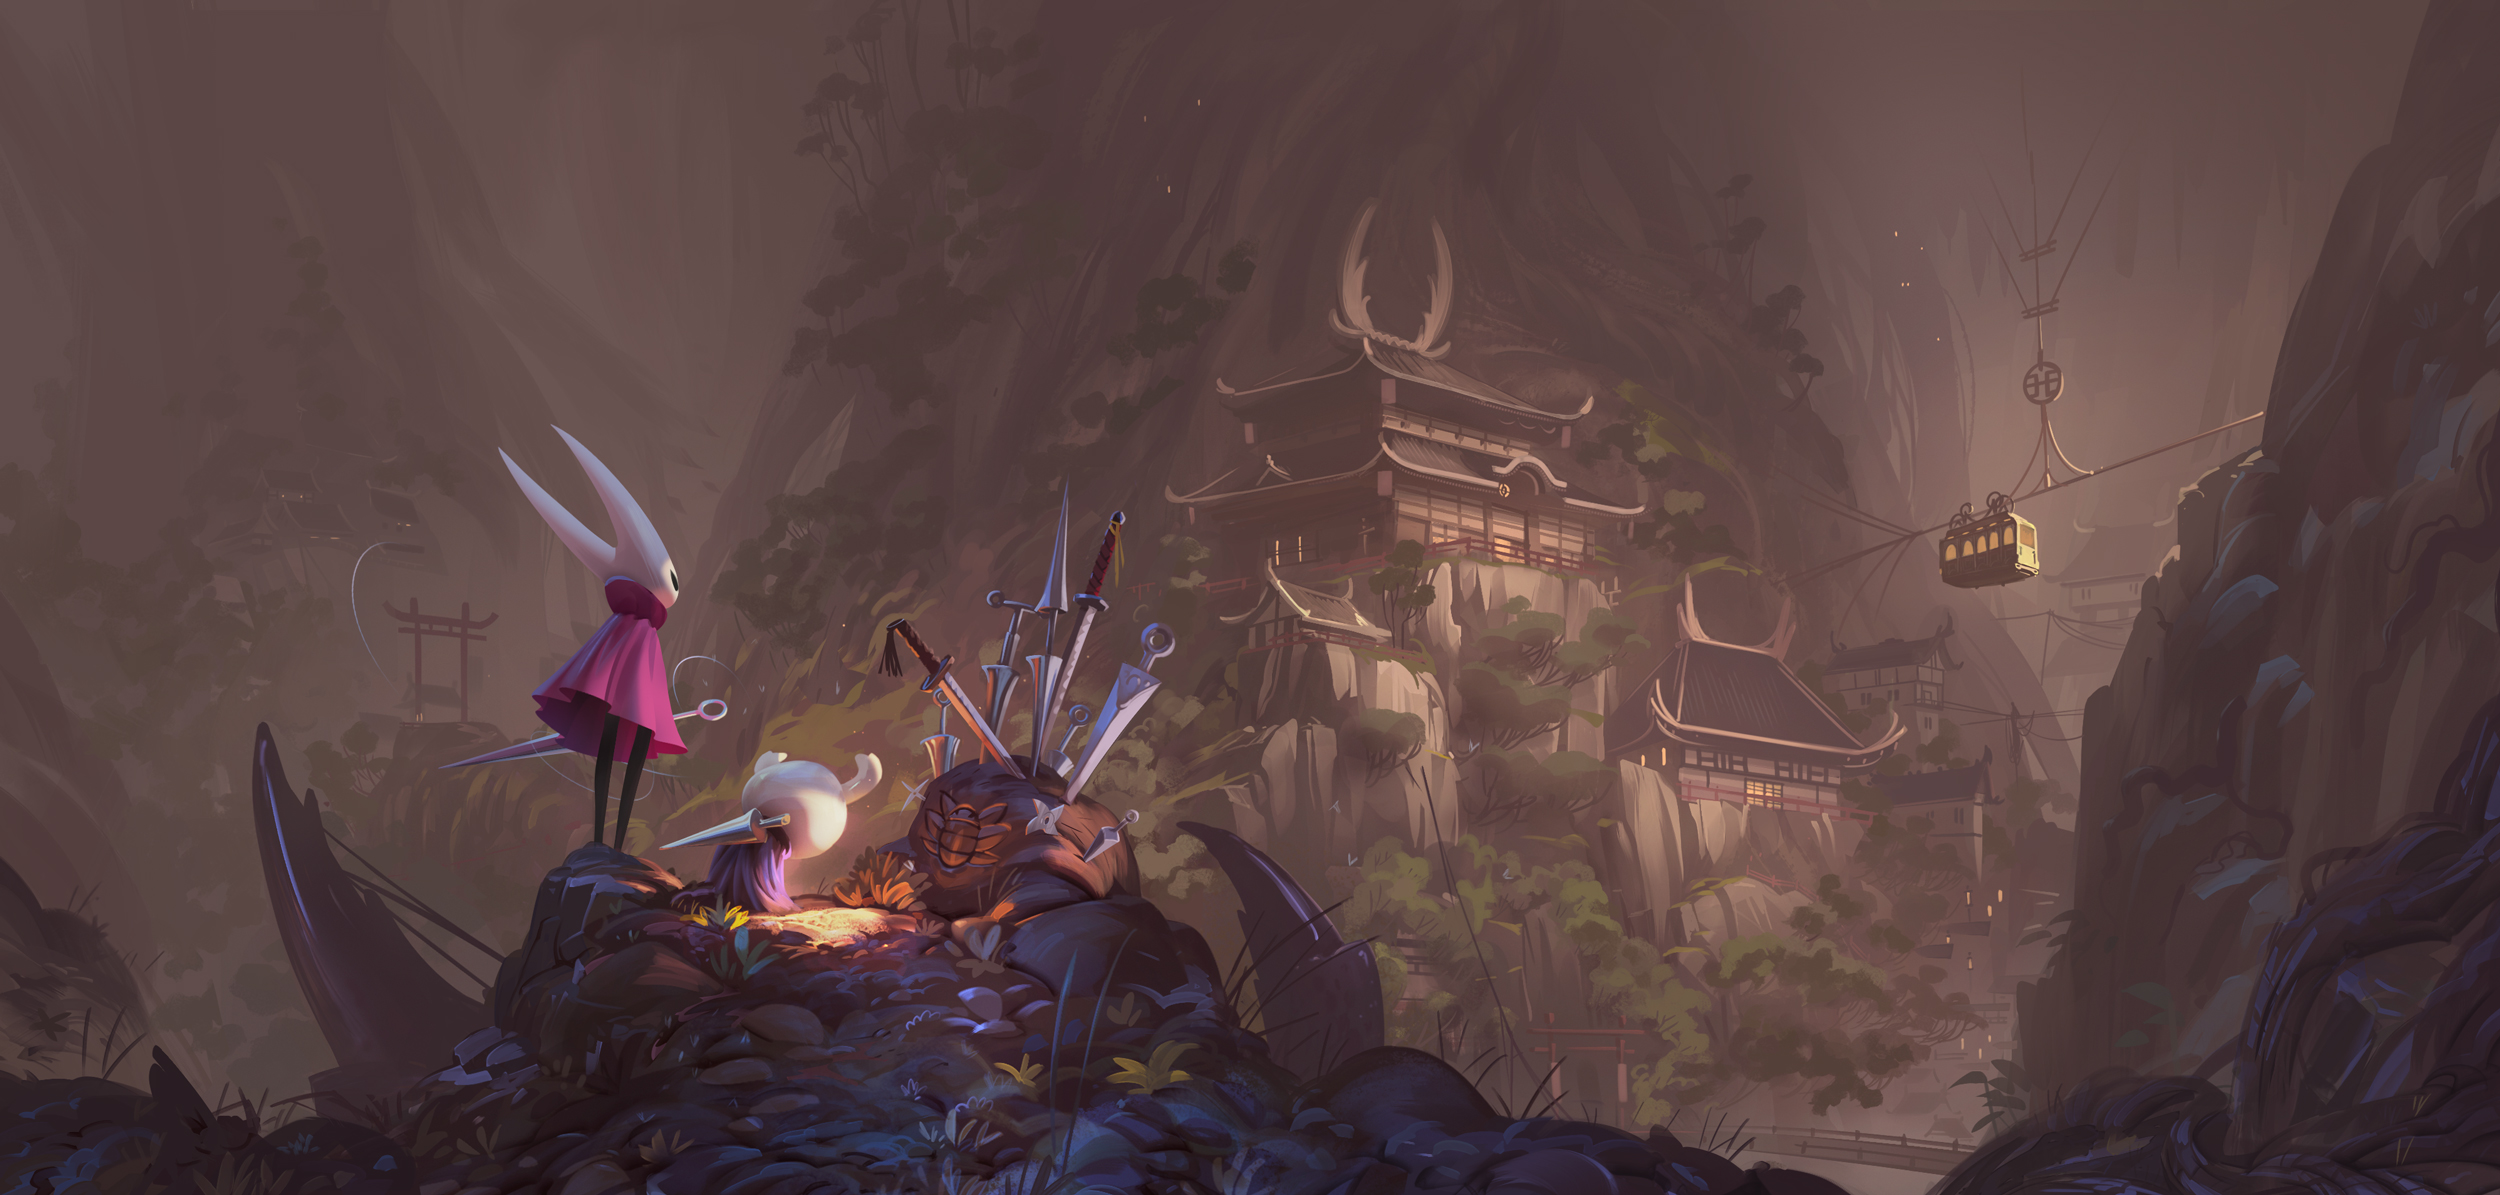
\includegraphics[scale=0.07]{pics/pic.jpg}
  }
  \hspace{30pt}
  \subfloat{
    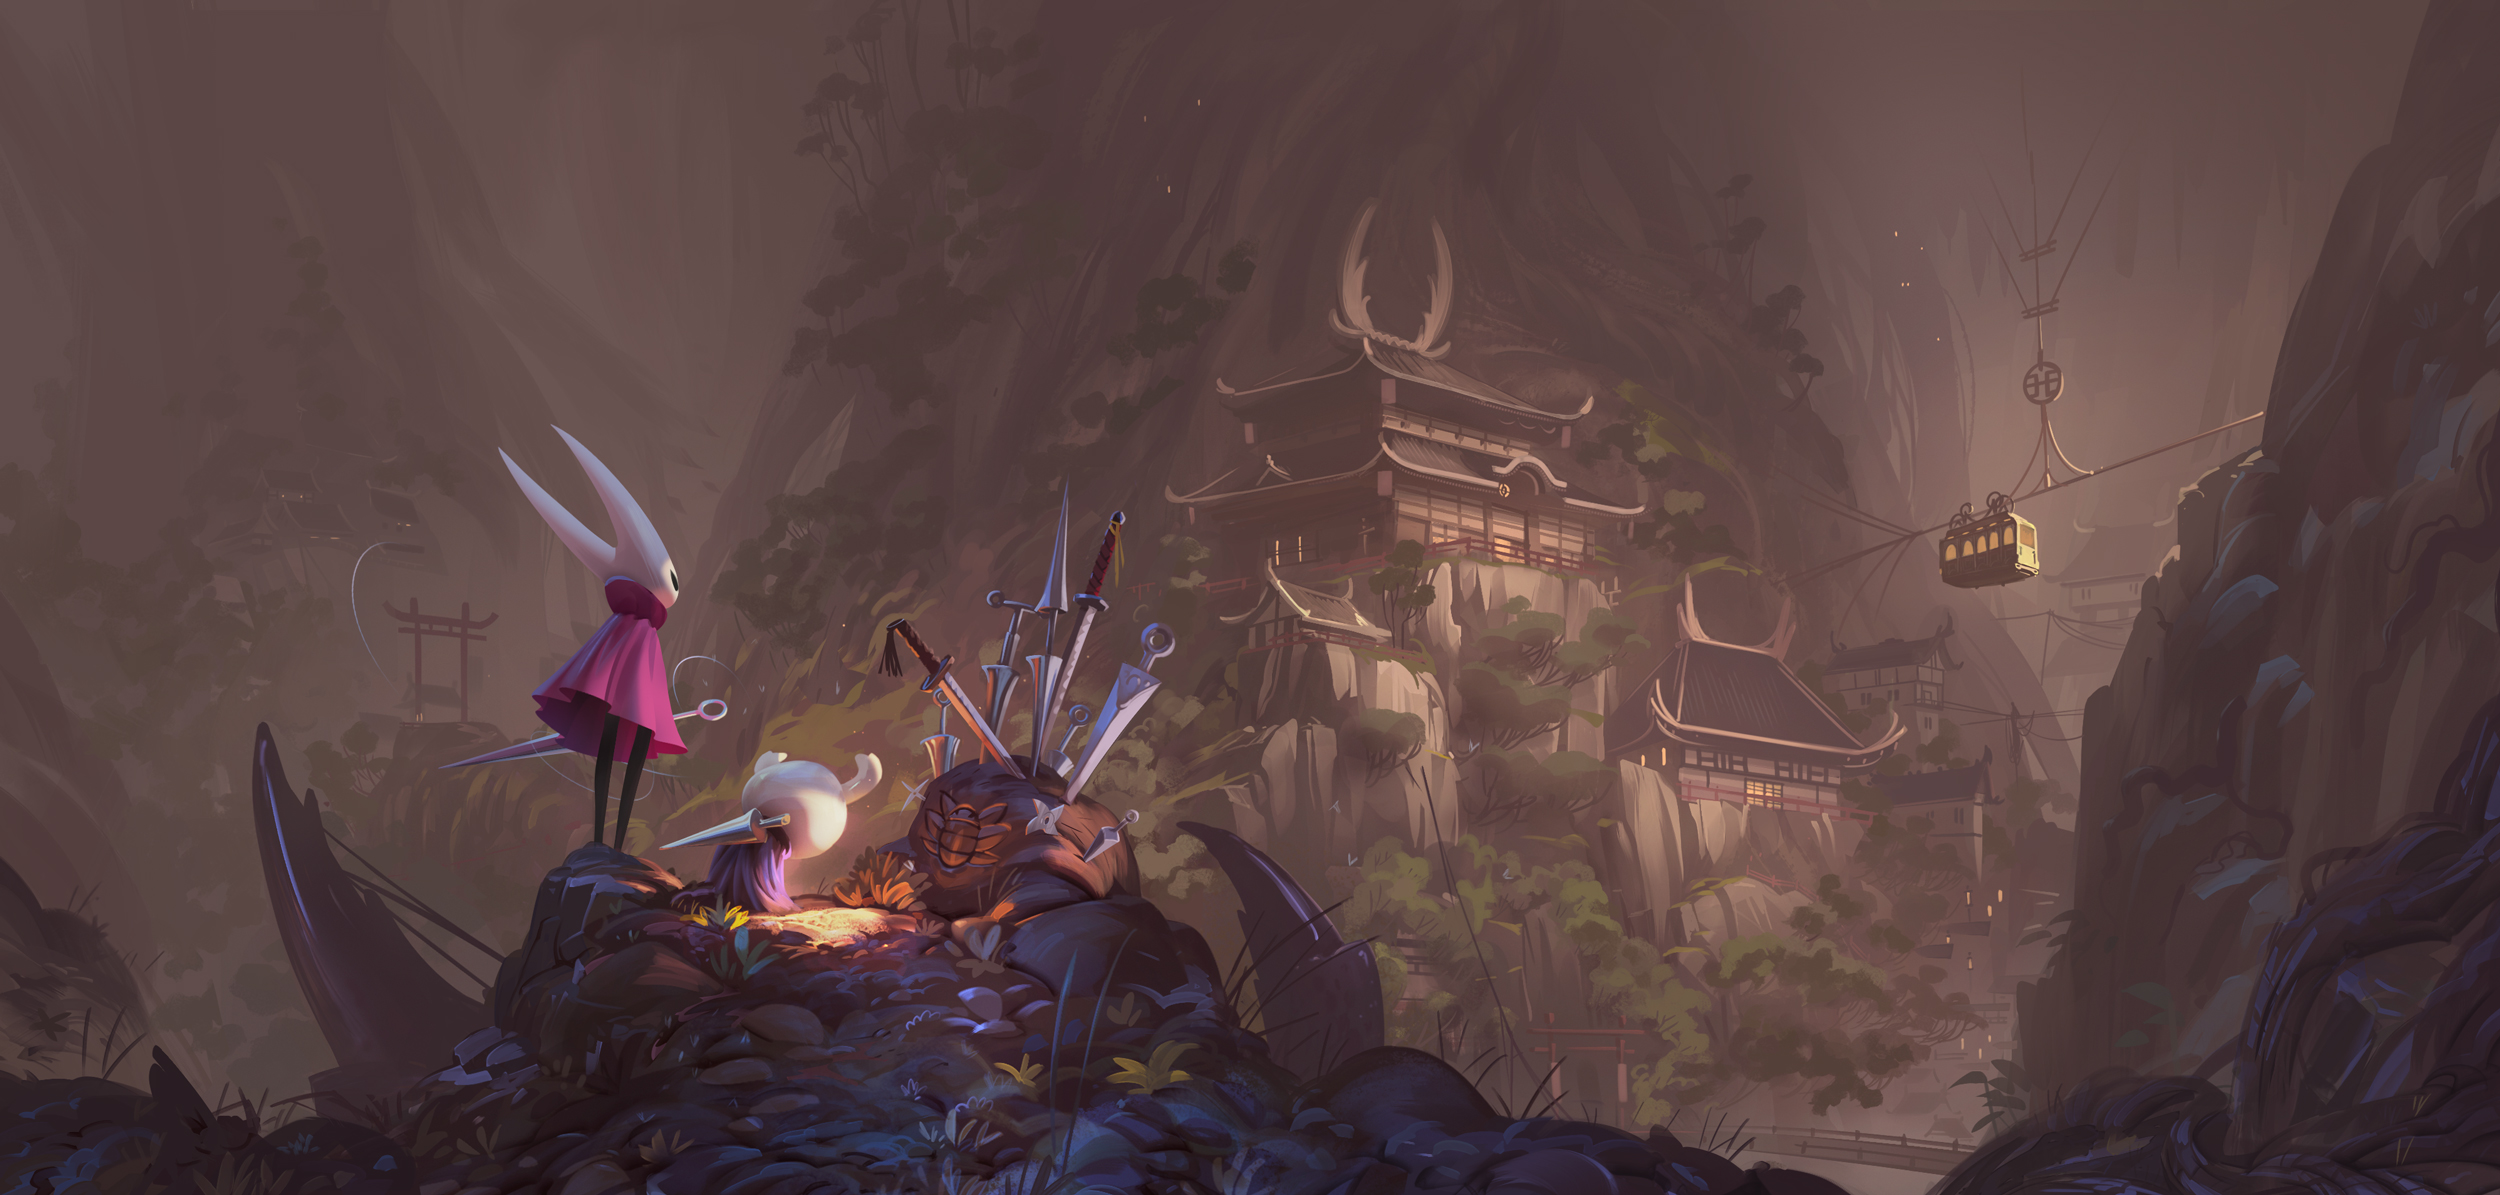
\includegraphics[scale=0.07]{pics/pic.jpg}
}
\caption{Hollow Knight}
\label{fig:HK}
\vspace{-0.3cm}
\end{figure}


\section{表格}
三线表的绘制。很多刊物都明确规定稿件中要使用三线表。三线表在必要时也可添加若干条水平辅助分隔中线。
\begin{table}[!h]
\centering
\caption{序号计数器及其用途\label{tab:2-1}}
\begin{tabular}{@{}ll@{}}
\toprule[1pt]
计数器名   & 用途            \\ \midrule
chapter    & 章序号计数器    \\
section    & 节序号计数器    \\
subsection & 小节序号计数器  \\
\bottomrule[1pt]
\end{tabular}
\end{table}

表\ref{tab:2-1}中列出了常用章节的计数器名称。

\section{列表}
排序列表
\begin{enumerate}
  \item item of the list.
  \item item of the list.
  \item item of the list.
\end{enumerate}



  % --- Reference | 参考文献 ---
  \bibliography{refs/reference}
  % --- Review | 审查表 ---
  % \reviewPage

  % ===== Appendix | 附录 =====
  % \appendix
  % %! TEX root = ../main.tex

\chapter{Appendx 1}
\appchapter{附录第一章}
\appsection{课题背景}
\lipsum[3]


  % \includepdf[pages={1,2}]{appendices/article.pdf}
\end{document}

